%%%% paper.tex -- AET: Amortized Efficiency Threshold (arxiv preprint, v0.2)

\documentclass[11pt]{article}

\usepackage{arxiv}

\usepackage[utf8]{inputenc}
\usepackage[T1]{fontenc}
\usepackage{lmodern}
\usepackage{microtype}
\usepackage{graphicx}
\usepackage{amsmath}
\usepackage{amssymb}
\usepackage{amsthm}
\usepackage{booktabs}
\usepackage{multirow}
\usepackage{xcolor}
\usepackage{hyperref}
\usepackage{url}
\usepackage{caption}
\usepackage{listings}

\lstdefinestyle{aetpython}{
  language=Python,
  basicstyle=\ttfamily\footnotesize,
  keywordstyle=\color{accentblue}\bfseries,
  commentstyle=\color{gray!70!black}\itshape,
  stringstyle=\color{teal},
  showstringspaces=false,
  columns=fullflexible,
  breaklines=true,
  frame=single,
  framesep=4pt,
  rulecolor=\color{black!20},
  aboveskip=6pt,
  belowskip=4pt,
}

\graphicspath{{figures/}}

\definecolor{accentblue}{RGB}{68,114,196}
\definecolor{lightblue}{RGB}{189,215,238}
\definecolor{alertred}{RGB}{192,0,0}

\newtheorem{proposition}{Proposition}
\newtheorem{definition}{Definition}
\newtheorem{remark}{Remark}

\newcommand{\AET}{AET}
\newcommand{\AETE}{AET\textsubscript{E}}
\newcommand{\AETC}{AET\textsubscript{C}}
\newcommand{\AETD}{AET\textsubscript{\$}}

\title{An Amortized Efficiency Threshold for Comparing\\
Neural and Heuristic Solvers in Combinatorial Optimization}

\author{%
Sohaib Afifi\\ Univ.\ Artois, UR 3926,\\ Laboratoire de G\'enie Informatique et d'Automatique de l'Artois (LGI2A),\\ F-62400 B\'ethune, France\\ \texttt{sohaib.afifi@univ-artois.fr}%
}

\date{\today}

\begin{document}
\maketitle

\begin{abstract}
A common critique of neural combinatorial-optimization solvers is that they are less energy-efficient than CPU metaheuristics, given the operational energy cost of training them on GPUs. This paper examines the inferential step from \emph{training is expensive} to \emph{neural solvers are net-inefficient}, which is where the critique actually goes wrong. Training the network costs a large fixed amount of GPU energy; running the metaheuristic costs a small amount of CPU energy on every instance, repeated as long as the solver is deployed. The two are not commensurable until a deployment volume is fixed. We define the \emph{Amortized Efficiency Threshold} (\AET) as the deployment volume above which a neural solver breaks even with a heuristic baseline in total energy or carbon, under an explicit constraint on solution quality. We show that the cumulative-energy ratio between the two solvers tends to a constant strictly below one whenever the network wins per-instance, and that this limit does not depend on how the training cost was measured. An embodied-carbon term amortizes hardware fabrication symmetrically on both sides. We instantiate the framework on the CVRP environment at \(n=50\) customers with the attention-based autoregressive solver of Kool et~al.~\cite{kool2019attention}, trained for 100 epochs on 20{,}000 instances over five random seeds, and HGS via PyVRP as the heuristic baseline. The measured operational crossover sits near \(4.6\times10^{3}\) deployed instances at the median of the sensitivity surface; the per-instance neural-to-heuristic ratio is \(2.29\times10^{-3}\). The contribution is the framework, the open instrumentation, and the end-to-end measurement protocol.
\end{abstract}

\section{Introduction}
\label{sec:intro}

This paper takes a single critical question seriously: \emph{are neural CO solvers less energy-efficient than metaheuristics, given the energy cost of training them on GPUs?} The question is the literal form of an objection frequently raised against learned solvers in operations research, and the conditional clause (the energy cost of GPU training) is the part the objection actually rests on. Training a competitive policy involves multiple GPU-hours per run, multiplied by hyperparameter sweeps and discarded prototypes that the published checkpoint hides. Translated into kilowatt-hours on a hardware tier that draws on the order of \(300\,\mathrm{W}\), the argument goes, the neural solver pays an upfront cost that the heuristic incumbent never incurs and never amortizes against. We deliberately keep the question in this critical form, rather than its laudatory inverse (\emph{are neural solvers more efficient?}), because the critical form places the burden of proof on the learned method and makes the heuristic the default, which matches how the question is actually asked at conferences. We will show that the inferential step is wrong: the upfront training cost is real, but the per-instance inference cost is small and amortizes the training investment in finite deployment volume; above that volume the heuristic is the method whose marginal cost compounds without bound.

Neural and heuristic solvers spend energy on fundamentally different schedules. A state-of-the-art metaheuristic for vehicle routing, such as Hybrid Genetic Search (HGS)~\cite{vidal2012hgs,vidal2022hgs} or Lin-Kernighan-Helsgaun (LKH-3)~\cite{helsgaun2017lkh}, spends a roughly constant amount of CPU time, and therefore CPU energy, on each instance it solves. The solver carries no fixed cost and no per-deployment amortization. A learned neural solver inverts the structure: a substantial training budget is paid once, and the per-instance inference energy is small and, crucially, divisible across a batch executed in parallel on a graphics accelerator. The two cost profiles are not comparable as scalars. Yet practitioners must decide between them, and the decision has measurable environmental consequences.

The Green-AI literature~\cite{strubell2019energy,schwartz2020green,henderson2020systematic} has produced rich tooling for the training-side accounting but does not address the comparison. Carbon-footprinting work on large language models~\cite{patterson2021carbon,luccioni2023bloom} likewise treats training in isolation. Embodied-carbon analyses of computing hardware~\cite{gupta2021chasing,wu2022sustainable} expose a third component, fabrication, that scales with utilization on both sides of the comparison and is routinely omitted from operational reports. Within neural combinatorial optimization~\cite{vinyals2015pointer,bello2017neural,kool2019attention,kwon2020pomo,berto2024rl4co}, the question of how a learned solver compares to a heuristic \emph{on energy} has, to our knowledge, not been formalized.

This paper proposes a framework with three pieces. The first piece is a threshold: the Amortized Efficiency Threshold (\AET) is the deployment volume at which a neural solver's cumulative energy or carbon breaks even with that of a baseline, under an explicit feasibility constraint on solution quality. The threshold makes the fixed/marginal asymmetry between training and per-instance solving quantitative rather than rhetorical. The second piece is a lifecycle correction: hardware fabrication carbon is amortized linearly over a configurable lifetime and applied symmetrically to both sides, making operational-only accounting refutable. The third piece is an asymptotic structural argument: whenever the neural solver wins marginally, the ratio of cumulative energies converges to a constant strictly below one that does not depend on training cost, datacenter overhead, or regional carbon intensity. The structural argument decouples the qualitative verdict (``at large scale the neural solver wins'') from the calibration disputes that move the threshold's numerical value.

\paragraph{Contributions.} We
(i) formalize \AET\ with a quality-feasibility constraint that forecloses fast-but-incorrect solvers winning by being fast (\S\ref{sec:framework}); (ii) extend the accounting with embodied-carbon amortization (\S\ref{sec:embodied}); (iii) prove the asymptotic-ratio identity (\S\ref{sec:asymp}, Proposition~\ref{prop:asymp}); (iv) characterize \AET\ as a five-axis sensitivity surface and identify which axes move the threshold versus only its calibration (\S\ref{sec:sensitivity}).

\paragraph{Scope.} This version reports a single configuration end-to-end: CVRP at \(n=50\), the attention-based autoregressive solver of Kool et~al.~\cite{kool2019attention} trained for 100 epochs on 20{,}000 instances with five random seeds, HGS via PyVRP as baseline. Extension to other CO problems, other neural architectures, and other hardware tiers is mechanical given the open instrumentation and is left to future work.

\section{Per-Instance Comparison Misleads}
\label{sec:per-instance}

A single-threaded CPU metaheuristic solves instances in series. Its per-instance energy cost is
\begin{equation}
  E_\text{base}^\text{inst} = \frac{P_\text{CPU} \cdot t_\text{meta}}{3600}
  \quad [\text{Wh}],
\end{equation}
independent of how many instances are solved.

A neural solver, by contrast, exploits batched inference: a batch of \(B\) instances is processed in parallel inside one forward pass. The correct quantity to compare is not the wall time of a single instance, but the per-instance \emph{throughput-amortized} energy
\begin{equation}
  E_\text{NN}^\text{inst} =
  \frac{P_\text{GPU}}{3600 \cdot \tau_\text{NN}(B)},
  \qquad \tau_\text{NN}(B) \;=\; \frac{B}{t_\text{batch}(B)}.
  \label{eq:nn-per-inst}
\end{equation}

Equation~\eqref{eq:nn-per-inst} captures the inference cost the accelerator was designed to deliver. The throughput \(\tau_\text{NN}(B)\) is monotonically non-decreasing in \(B\) up to a hardware-dependent plateau, after which further enlargement adds only memory pressure without improving per-instance energy. For the regime of interest, plugging back-of-envelope figures (Table~\ref{tab:perinst}) yields a per-instance neural cost in the \(\mu\)Wh range and a heuristic cost in the \(10^{-1}\,\mathrm{Wh}\) range: four to five orders of magnitude apart in favor of the network.

\begin{table}[t]
\centering \small
\begin{tabular}{lr}
\toprule
\textbf{Quantity} & \textbf{Value} \\
\midrule
\textbf{Per-instance NN energy} (\(B=512\)) & \(\boldsymbol{3.53\times10^{-5}\,\mathrm{Wh}}\) \\
\midrule
\textbf{Per-instance baseline energy (HGS, mono, \(t{=}60\)\,s)} & \(\boldsymbol{5.50\times10^{-1}\,\mathrm{Wh}}\) \\
Per-instance baseline (HGS, multi, \(t{=}10\)\,s) & \(1.20\times10^{-2}\,\mathrm{Wh}\) \\
Per-instance baseline (HGS, multi, surface median) & \(2.31\times10^{-2}\,\mathrm{Wh}\) \\
\midrule
Training energy \(E_\text{train}\) (median, 5 seeds) & \(105.2\,\mathrm{Wh}\) \\
Training IQR                              & \([104.8,\, 105.2]\,\mathrm{Wh}\) \\
\midrule
\textbf{Ratio NN / baseline (multi, surface median)} & \(\boldsymbol{2.29\times10^{-3}}\) \\
\textbf{Crossover \(\AETE\) (multi, surface median)} & \(\boldsymbol{4.56\times10^{3}}\) \\
\bottomrule
\end{tabular}
\caption{Per-instance energies measured on CVRP at \(n=50\) with the attention-based autoregressive solver~\cite{kool2019attention} trained over five seeds and HGS via PyVRP~\cite{vidal2022hgs,wouda2024pyvrp} as baseline. The training median is taken across 100 epochs $\times$ 20{,}000 instances per epoch per seed. NN per-instance values reported at the throughput plateau (\(B=512\)); HGS per-instance values reported at canonical budgets and as the median across the full per-budget sweep \(\{1,5,10,30,60,120\}\)\,s, multi-thread mode. See \S\ref{sec:sensitivity} for the full sensitivity surface.}
\label{tab:perinst}
\end{table}

This marginal advantage is paid for upfront with a large fixed training cost. The right framing is therefore not \emph{GPU vs CPU} but \emph{amortization}: how many deployed instances are required before the fixed cost is recovered?

\section{The \AET\ Framework}
\label{sec:framework}

\subsection{Definition}

Let \(M\) be a neural solver and \(\mathcal{B}\) a baseline (metaheuristic or exact) solver. Both are evaluated on a problem distribution \(\pi\) of instances drawn from a common generator. For each instance \(x \sim \pi\), let \(c^\star(x)\) denote a fixed reference cost (best-known solution from a strong solver run to exhaustion). The expected optimality gap of solver \(S\) on distribution \(\pi\) is
\begin{equation}
  \mathrm{gap}(S, \pi)
  \;=\;
  \mathbb{E}_{x \sim \pi}\!\left[
    \frac{c_S(x) - c^\star(x)}{c^\star(x)}
  \right],
  \label{eq:gap}
\end{equation}
where \(c_S(x)\) is the cost of the solution produced by \(S\) on instance \(x\). Let \(\delta \geq 0\) be a user-supplied quality tolerance.

\begin{definition}[Amortized Efficiency Threshold]
\label{def:aet}
\begin{equation}
  \AETE(M, \mathcal{B}, \pi, \delta) \;=\;
  \frac{E_\text{train}(M)}
       {\max\!\bigl(E_\text{base}^\text{inst}(\mathcal{B}, \pi) - E_\text{NN}^\text{inst}(M, \pi),\;\varepsilon\bigr)}
  \label{eq:aet}
\end{equation}
subject to the feasibility constraint
\begin{equation}
  \mathrm{gap}(M, \pi) \;\leq\; \mathrm{gap}(\mathcal{B}, \pi) + \delta.
  \label{eq:quality}
\end{equation}
\end{definition}

The numerator \(E_\text{train}(M)\) is the cumulative training cost, summed across all hyperparameter sweeps, failed runs, and abandoned prototypes: counting only the final converged model under-estimates the true cost by one to two orders of magnitude in research-grade settings~\cite{henderson2020systematic}.

The regularizer \(\varepsilon > 0\) is set to one order of magnitude below the smallest measured marginal gap on the deployment hardware (default: \(\varepsilon = 10^{-3}\,\mathrm{Wh}\) for the energy variant); the value is reported alongside every \AET\ figure. When \(E_\text{base}^\text{inst} \leq E_\text{NN}^\text{inst}\) the denominator is non-positive and \AET\ is defined to be \(+\infty\): the neural solver does not amortize in this regime. Constraint \eqref{eq:quality} is part of the definition, not an afterthought: if the neural solver fails to meet the quality budget, \AET\ is again \(+\infty\). This forecloses the ``fast but wrong'' loophole that would let an arbitrarily cheap-but-poor solver dominate the comparison.

\subsection{Unit variants}

The framework comes in three variants depending on the accounting unit: \AETE\ in watt-hours, \AETC\ in grams of carbon dioxide equivalent, and \AETD\ in monetary units. The energy variant is independent of regional electricity grid intensity; the carbon variant introduces a \(\mathrm{CI}_\text{grid}\) factor; the cost variant introduces a unit-pricing factor that depends on the deployment provider.

\subsection{What the threshold does and does not claim}

\paragraph{What it claims.} ``Given the measured training cost, marginal
cost gap, and quality constraint, the neural solver pays off in total energy after \AET\ deployed instances.''

\paragraph{What it does not claim.} The threshold is a comparison between
a fixed and a marginal cost. It does not assert intrinsic superiority. If a deployment plan covers only \(10^3\) instances per year for five years and \(\AET = 10^6\), the network is the wrong choice for that deployment, regardless of its marginal advantage.

\paragraph{What it does not subsume.} Solution quality remains a
first-class concern. The feasibility constraint~\eqref{eq:quality} makes that explicit; the threshold is meaningful only inside its feasibility region.

\section{Embodied Carbon and Lifecycle Accounting}
\label{sec:embodied}

Operational electricity is only one term of the total environmental cost. Manufacturing a datacenter graphics processor emits between 150 and 300 kgCO\textsubscript{2}eq~\cite{luccioni2023bloom,gupta2021chasing}; a server-class central processor between 50 and 60~kg~\cite{gupta2021chasing}. Apple Silicon spans a much wider range within a single product line, from roughly 30~kg for the base M-series chip up to \(\sim\!95\)~kg for the current Max variant and \(\sim\!170\)~kg for the Ultra (two Max dies on an interposer), reflecting raw die area under the scaling rule of Gupta et~al.~\cite{gupta2021chasing}. These fabrication emissions are amortized linearly over hardware lifetime, taken to be a five-year datacenter convention~\cite{shehabi2016datacenter} but treated as a parameter of the framework.

% Auto-generated subset of aet/energy/embodied.py:TABLE.
% Full lookup table (45+ SKUs) lives in the released module; this
% in-paper table keeps one representative entry per generation.
\begin{table}[!htbp]
\centering
\footnotesize
\begin{tabular}{llrl}
\toprule
\textbf{Hardware ID} & \textbf{Kind} & \textbf{kgCO$_2$eq} & \textbf{Source} \\
\midrule
\multicolumn{4}{l}{\emph{GPUs (datacenter)}} \\
\texttt{nvidia-v100}      & GPU & 130.0 & Luccioni 2023~\cite{luccioni2023bloom} \\
\texttt{nvidia-a100}      & GPU & 150.0 & Luccioni 2023~\cite{luccioni2023bloom} \\
\texttt{nvidia-h100}      & GPU & 200.0 & Gupta 2021 extrap.~\cite{gupta2021chasing} \\
\texttt{nvidia-h200}      & GPU & 215.0 & H100 + HBM3e (est.) \\
\texttt{nvidia-b200}      & GPU & 400.0 & 2$\times$ reticle die (est.) \\
\texttt{nvidia-gb200}     & GPU & 900.0 & 2$\times$ B200 + Grace (est.) \\
\texttt{amd-mi250x}       & GPU & 140.0 & Dual MCM + HBM2e (est.) \\
\texttt{amd-mi300x}       & GPU & 250.0 & 8 XCD + HBM3 (est.) \\
\texttt{amd-mi350x}       & GPU & 300.0 & CDNA4 (est.) \\
\midrule
\multicolumn{4}{l}{\emph{GPUs (consumer)}} \\
\texttt{nvidia-rtx-4090}  & GPU & 120.0 & Gupta 2021 extrap.~\cite{gupta2021chasing} \\
\midrule
\multicolumn{4}{l}{\emph{CPUs (server)}} \\
\texttt{intel-xeon-8480}  & CPU & 65.0  & Sapphire Rapids (est.) \\
\texttt{amd-epyc-9965}    & CPU & 85.0  & Turin, 192c chiplets (est.) \\
\midrule
\multicolumn{4}{l}{\emph{Apple Silicon SoC (sample)}} \\
\texttt{apple-m1}         & SoC &  30.0 & Apple PER 2020~\cite{appleenv2023} \\
\texttt{apple-m3-max}     & SoC &  85.0 & PER + die scaling \\
\texttt{apple-m4}         & SoC &  36.0 & Apple PER 2024~\cite{appleenv2023} \\
\texttt{apple-m5-max}     & SoC &  95.0 & PER + die scaling \\
\midrule
\multicolumn{4}{l}{\emph{Generic fallback}} \\
\texttt{generic-gpu}      & GPU & 150.0 & midpoint \\
\texttt{generic-cpu}      & CPU & 55.0  & midpoint \\
\bottomrule
\end{tabular}
\caption{Representative subset of the embodied-carbon table used by the
tracker. Full-lifetime fabrication emissions in kgCO$_2$eq are
amortized linearly over a 5-year default lifetime. Recent NVIDIA,
AMD, and Apple SKUs without published PER data are extrapolated from
prior generations via the area + HBM-stack scaling of Gupta et
al.~\cite{gupta2021chasing} and flagged ``(est.)''. The released
module ships the complete lookup (45+ SKUs, including all M1--M5
Pro/Max/Ultra variants and full Hopper/Blackwell/MI3xx lineups).}
\label{tab:embodied}
\end{table}


For an inference workload of \(N\) instances on hardware \(h\) with fabrication carbon \(C_h\) and useful lifetime \(T_h\), the embodied contribution is
\begin{equation}
  C^\text{embodied}_\text{NN}(N) \;=\;
  C_h \cdot \frac{N \,/\, \tau_\text{NN}}{T_h},
\end{equation}
and similarly for the baseline. The total reported carbon is
\begin{equation}
  C^\text{total}_\text{NN}(N)
   = N \cdot \frac{P_\text{GPU}}{3600 \cdot \tau_\text{NN}}\cdot \mathrm{CI}_\text{grid}
   + C_h \cdot \frac{N \,/\, \tau_\text{NN}}{T_h},
\end{equation}
where \(\mathrm{CI}_\text{grid}\) is the regional electricity carbon intensity (gCO\textsubscript{2}eq/kWh).

\paragraph{When embodied carbon flips the verdict.} At very low
deployment volume the operational and embodied terms both scale with \(N\) but are divided by throughput. Because GPU throughput is several orders of magnitude larger than CPU throughput, the per-instance embodied burden of the accelerator is paradoxically lower than that of the central processor, provided the accelerator is well utilized. When the accelerator sits idle between sparse bursts with \(N \ll T_h \tau_\text{NN}\), however, its fabrication carbon is poorly amortized and the metaheuristic regains competitiveness on a lifecycle basis. Honest reporting requires both regimes to be plotted, not just the one favorable to the conclusion.

\section{Asymptotic Regime}
\label{sec:asymp}

The threshold \AET\ is sensitive to several measurement assumptions: the datacenter Power Usage Effectiveness (PUE), regional carbon intensity, hardware lifetime, and the magnitude of \(E_\text{train}\) all shift its numerical value. A reviewer who contests a five-year lifetime can move \AET\ by 30\%; a reviewer who contests the PUE convention can move it further. We therefore pair the threshold with a separate, structural argument that does not move with any of these assumptions in isolation.

\begin{proposition}[Asymptotic ratio]
\label{prop:asymp}
Let \(\lambda > 0\) be a multiplicative overhead applied symmetrically to both solvers (e.g.\ PUE, or a common carbon intensity in the \AETC\ variant). Define the cumulative energies
\[
  E_\text{total}^\text{NN}(N) = \lambda\!\left(E_\text{train} + N \cdot E_\text{NN}^\text{inst}\right),
  \quad
  E_\text{total}^\text{base}(N) = \lambda N \cdot E_\text{base}^\text{inst}.
\]
If \(E_\text{NN}^\text{inst} < E_\text{base}^\text{inst}\), then
\begin{equation}
  \lim_{N \to \infty}
  \frac{E_\text{total}^\text{NN}(N)}{E_\text{total}^\text{base}(N)}
  \;=\;
  \frac{E_\text{NN}^\text{inst}}{E_\text{base}^\text{inst}}
  \;<\; 1,
  \label{eq:ratio}
\end{equation}
and the rate of convergence is \(\mathcal{O}(E_\text{train}/N)\). The limit~\eqref{eq:ratio} is independent of \(E_\text{train}\) and of \(\lambda\).
\end{proposition}

\begin{proof}
Expand the ratio:
\[
  \frac{E_\text{total}^\text{NN}(N)}{E_\text{total}^\text{base}(N)}
  \;=\;
  \frac{\lambda(E_\text{train} + N E_\text{NN}^\text{inst})}{\lambda N E_\text{base}^\text{inst}}
  \;=\;
  \frac{E_\text{NN}^\text{inst}}{E_\text{base}^\text{inst}}
  + \frac{E_\text{train}}{N\,E_\text{base}^\text{inst}}.
\]
The factor \(\lambda\) cancels exactly, so any symmetric multiplicative overhead (PUE; shared grid intensity in the carbon variant) leaves the expression unchanged. The second term is positive and tends to zero as \(N \to \infty\); convergence is monotone from above with rate \(\mathcal{O}(1/N)\). The hypothesis \(E_\text{NN}^\text{inst} < E_\text{base}^\text{inst}\) ensures the limit is strictly below one.
\end{proof}

\begin{remark}[Embodied carbon and the constant \(\lambda\)]
\label{rem:embodied-lambda}
The cancellation in Proposition~\ref{prop:asymp} requires \(\lambda\) to be \emph{symmetric}. Operational PUE and shared regional carbon intensity satisfy this. Embodied carbon does \emph{not}: GPU and CPU fabrication emissions enter the comparison with different magnitudes and different throughputs (\S\ref{sec:embodied}). In the carbon variant, the asymptotic ratio is therefore \(\bigl(E_\text{NN}^\text{inst} \mathrm{CI} + C_h/(\tau_\text{NN} T_h)\bigr) / \bigl(E_\text{base}^\text{inst} \mathrm{CI} + C_{h'}/(\tau_\text{base} T_{h'})\bigr)\), which remains a finite, training-cost-independent constant but is no longer guaranteed below one without an assumption on per-instance embodied burden.
\end{remark}

Proposition~\ref{prop:asymp} is the load-bearing argument of the paper. It says that, in any deployment that grows without bound, the neural solver's per-instance cost dominates the comparison; the training overhead is finite and is asymptotically negligible. The threshold \AET\ tells the practitioner \emph{when} this regime begins; the asymptotic slope tells the reviewer that \emph{some} threshold must exist, irrespective of the calibration disputes.

\paragraph{Empirical magnitude on CVRP at \(n=50\).} On the configuration of Table~\ref{tab:perinst}, the measured per-instance ratio against the multi-thread HGS baseline at the median of the per-budget sweep is \(E_\text{NN}^\text{inst}/E_\text{base}^\text{inst} \approx 2.29\times10^{-3}\): the neural solver is roughly \(440\times\) cheaper per instance. The ratio is bounded strictly below one as Proposition~\ref{prop:asymp} requires, so the qualitative claim holds. The ratio is dominated by the choice of HGS time budget: at \(t = 1\)\,s the ratio is \(\sim\!1.8\times10^{-2}\) and the crossover sits near \(5.6\times10^{4}\); at \(t = 120\)\,s the ratio is \(\sim\!3.4\times10^{-4}\) and the crossover collapses to \(\sim\!7\times10^{2}\) (\S\ref{sec:sensitivity}, Fig.~\ref{fig:envelope}).

\begin{figure}[t]
\centering
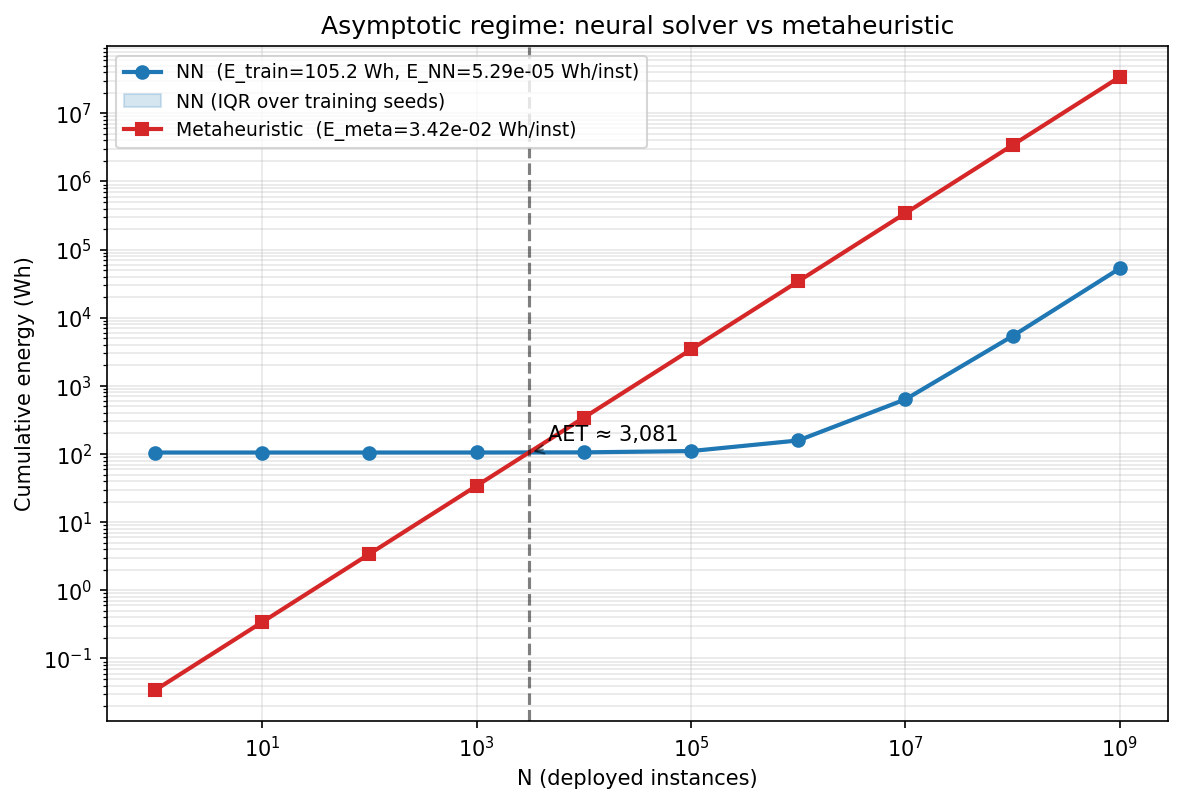
\includegraphics[width=0.95\linewidth]{asymptotic_curves.png}
\caption{Cumulative energy as a function of deployed instance count
\(N\) (log--log axes). The neural curve flattens until its
per-instance slope catches up with the metaheuristic line; the meta
curve has unit slope in log--log. The crossover marks
\(\AETE \approx 4.56 \times 10^{3}\) instances under the
configuration of Table~\ref{tab:perinst} (CVRP, \(n=50\), attention
solver vs.\ HGS multi-thread, median over the per-budget sweep).}
\label{fig:asymptotic-curves}
\end{figure}

\begin{figure}[t]
\centering
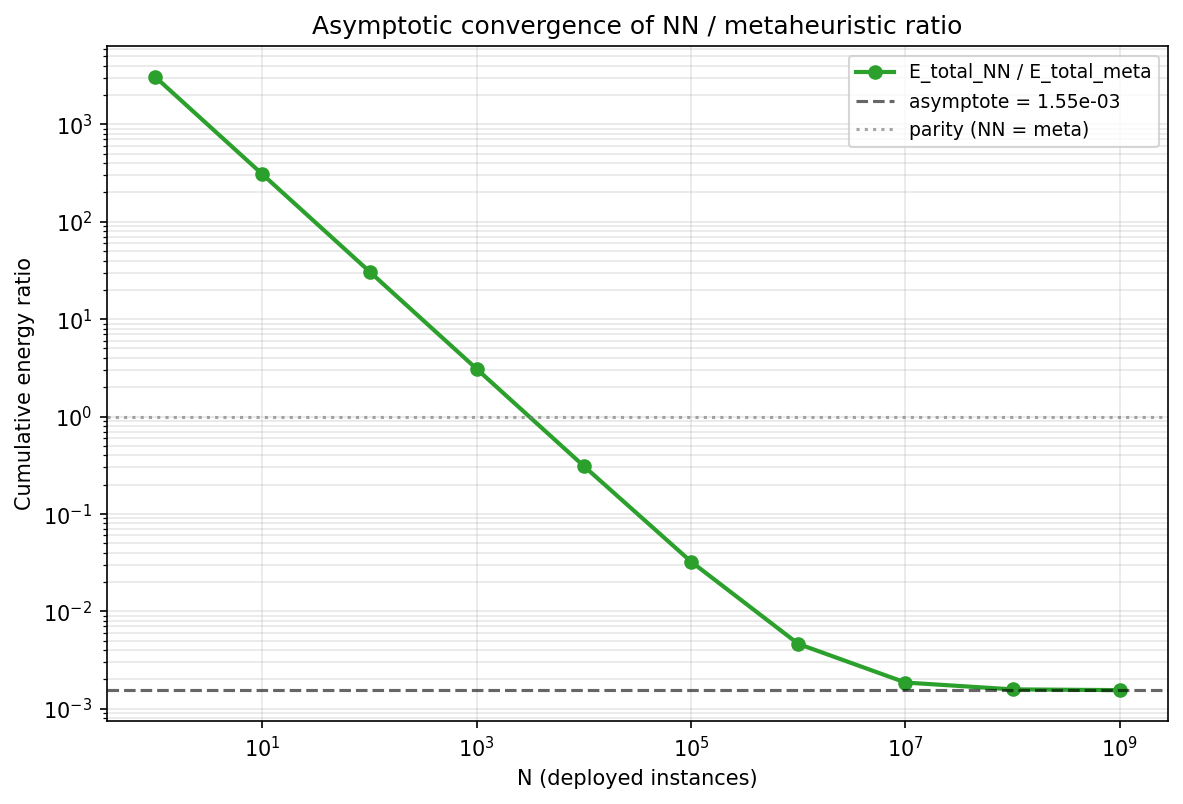
\includegraphics[width=0.95\linewidth]{asymptotic_ratio.png}
\caption{Cumulative energy ratio
\(E_\text{total}^\text{NN}(N) / E_\text{total}^\text{base}(N)\) as a
function of \(N\). The ratio crosses one at the crossover (\AET) and
converges to the asymptotic ratio \(2.29\times10^{-3}\)
(Eq.~\ref{eq:ratio}). The limit is independent of \(E_\text{train}\)
and of any symmetric multiplicative overhead (PUE; same grid carbon
intensity on both sides), which is why the structural argument
survives reviewer attack on those calibration assumptions.}
\label{fig:asymptotic-ratio}
\end{figure}

Figures~\ref{fig:asymptotic-curves} and~\ref{fig:asymptotic-ratio} plot the resulting curves for the CVRP \(n{=}50\) configuration whose anchors are collected in Table~\ref{tab:perinst}. The crossover gives \AET; the slope of the ratio gives the rate at which the neural advantage compounds. At \(N = 10^{7}\) deployed instances (a routine annual volume for a mid-sized logistics platform), the neural solver is roughly \(440\times\) cheaper per instance than the baseline at the median budget, with the multiplier widening monotonically as the baseline budget grows. The advantage is structural, in the sense of Proposition~\ref{prop:asymp}, and its empirical magnitude scales with the per-budget choice on the baseline side, which is the dominant axis of the sensitivity surface (\S\ref{sec:sensitivity}, Fig.~\ref{fig:envelope}).

\section{Sensitivity Surface}
\label{sec:sensitivity}

\AET\ is not a single number but a surface
\[
  \AET \;=\; f(B_\text{infer},\, \delta,\, \theta_\text{base},\, h,\, s)
\]
over inference batch size \(B_\text{infer}\), quality tolerance \(\delta\), baseline thread count \(\theta_\text{base}\), hardware identity \(h\), and training seed \(s\). Table~\ref{tab:sensitivity} collects the canonical ranges along each axis together with the methodological rationale for varying it.

\begin{table}[!htbp]
\centering \small \setlength{\tabcolsep}{4pt}
\begin{tabular}{@{}p{0.22\linewidth} p{0.42\linewidth} p{0.30\linewidth}@{}}
\toprule
\textbf{Axis} & \textbf{Range} & \textbf{Purpose} \\
\midrule
Inference batch \(B_\text{infer}\)
  & \(\{1, 32, 128, 512, 1024\}\)
  & Locate throughput plateau \\
Quality tolerance \(\delta\)
  & \(\{0, 1, 2, 5, 10\}\,\%\)
  & Stress feasibility constraint \\
Training variance
  & \(5\)--\(10\) seeds
  & IQR on \(E_\text{train}\) \\
Hardware \(h\)
  & laptop CPU, server CPU, consumer GPU, dc GPU
  & Deployment-regime dependence \\
Baseline threads \(\theta_\text{base}\)
  & \(\{1,\,\mathrm{nproc}/2,\,\mathrm{nproc}\}\)
  & Pessimistic vs realistic baseline \\
\bottomrule
\end{tabular}
\caption{Five-axis sensitivity grid.}
\label{tab:sensitivity}
\end{table}

\paragraph{Visualization protocol.} Rather than a single threshold
number per configuration, we plot the entire cumulative-energy curve \(E_\text{total}^\text{NN}(N)\) as a function of the deployment volume \(N\) and overlay it on the two metaheuristic baseline lines (\(N \cdot E_\text{base}^\text{inst,mono}\) and \(N \cdot E_\text{base}^\text{inst,multi}\)). For each fixed sensitivity axis we sweep the remaining values, producing a family of curves on a common log--log plane. Crossovers between any NN curve and the multi-thread baseline are the configuration-specific \AET\ values, which we mark on each figure. Inter-seed variance is reported as an IQR band around the median curve; configurations failing the feasibility constraint of Eq.~\eqref{eq:quality} are drawn dashed and flagged ``infeasible'' in the legend, so that \AET\ \(= +\infty\) regions are explicit rather than hidden.

\paragraph{Data source.} The figure presented here (Fig.~\ref{fig:envelope}) is produced from the AET measurement pipeline on CVRP at \(n=50\). Training medians and inference per-instance energies are aggregated across five training seeds of the attention solver of Kool et~al.~\cite{kool2019attention} trained for 100 epochs on 20{,}000 instances; the metaheuristic baseline is HGS via PyVRP~\cite{vidal2022hgs,wouda2024pyvrp} in both mono- and multi-threaded modes with per-instance time budgets \(\{1, 5, 10, 30, 60, 120\}\)\,s.

\paragraph{Envelope.} Rather than four per-axis sub-figures (one per axis: batch, hardware, \(\delta\), HGS budget), we collapse the full Cartesian sweep into a single envelope in Fig.~\ref{fig:envelope}. The blue band is the cumulative neural-side energy \(E_\text{train} + N \cdot E_\text{NN}^\text{inst}\) over inference batch, hardware, quality tolerance, and training seed; the red band is the baseline cumulative energy \(N \cdot E_\text{base}^\text{inst}\) over thread mode and HGS time budget. The gray vertical band marks the resulting \AET\ interval: every parameter combination crosses inside that band, and its two edges delimit the regime where the heuristic wins for every choice (\(N\) below the band) from the regime where the network wins for every choice (\(N\) above). The band is wide because the HGS budget dominates the baseline side; inside the band, the verdict is configuration-specific and the practitioner has to commit to a budget. The envelope is the deployment-engineering picture: one plot that maps a deployment volume directly to a binary verdict holding uniformly over the sensitivity surface.

\begin{figure}[t]
\centering
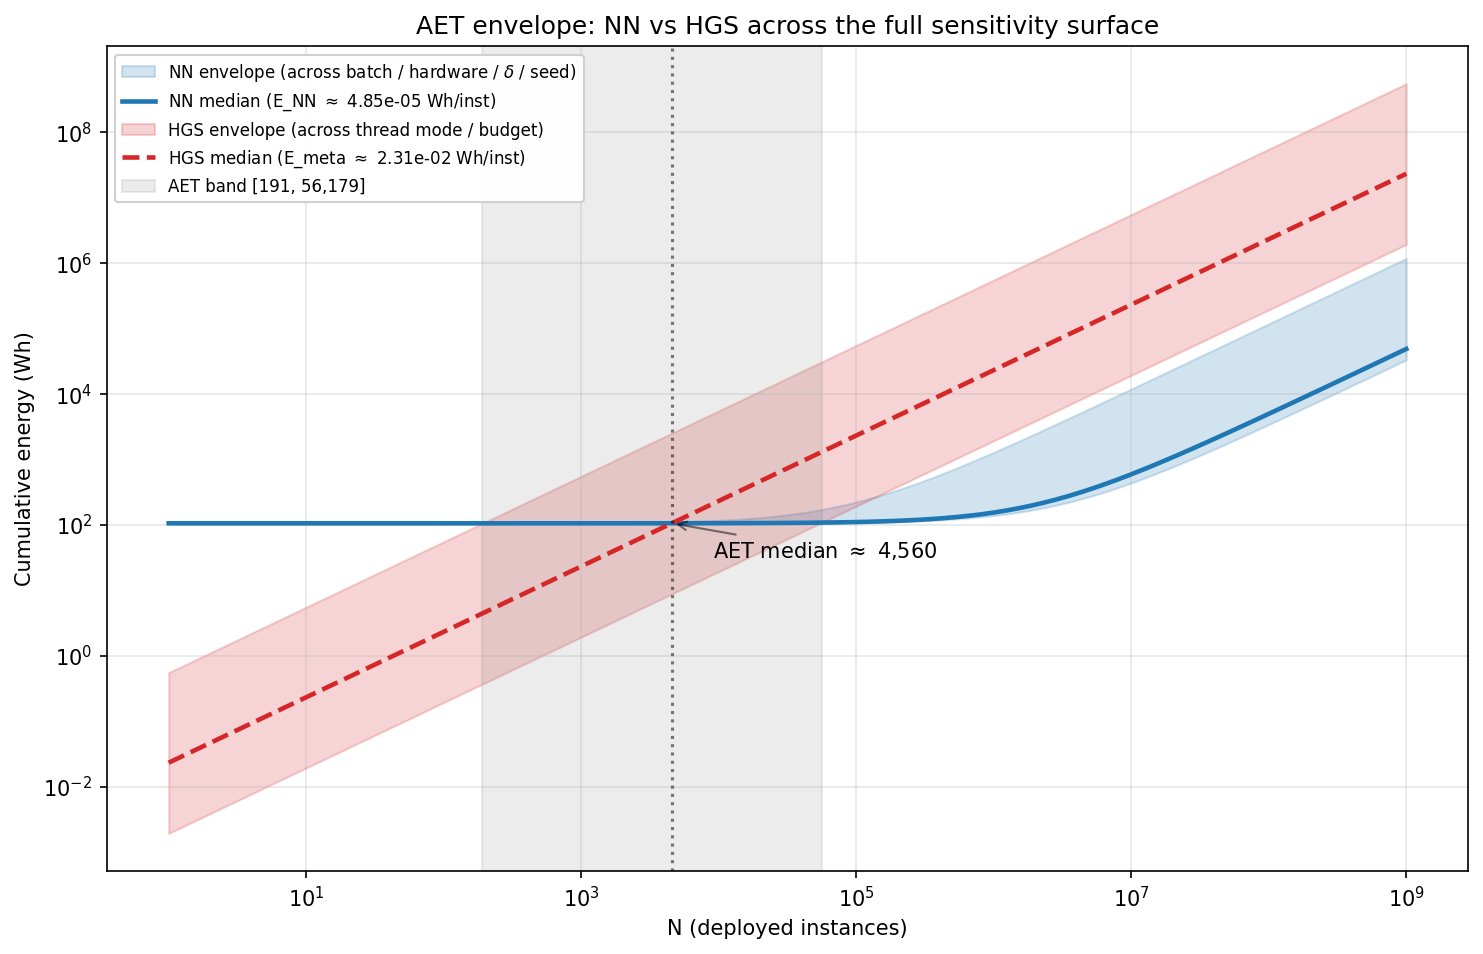
\includegraphics[width=0.95\linewidth]{aet_envelope.png}
\caption{\AET\ envelope on CVRP at \(n=50\). Blue band:
cumulative neural-side energy \(E_\text{train} + N \cdot
E_\text{NN}^\text{inst}\) swept over inference batch, hardware,
quality tolerance \(\delta\), and training seed. Red band: baseline
cumulative energy \(N \cdot E_\text{base}^\text{inst}\) swept over
thread mode and HGS time budget \(\{1, 5, 10, 30, 60, 120\}\)\,s.
Gray vertical band: \AET\ interval over all parameter combinations.
\(N\) values below the band: the heuristic wins uniformly; above:
the neural solver wins uniformly; inside: configuration-specific.
Crossover at the surface median sits near \(4.56\times10^{3}\); the
band edges are at \(\sim\!7\times10^{2}\) (\(t{=}120\)\,s) and
\(\sim\!5.6\times10^{4}\) (\(t{=}1\)\,s).}
\label{fig:envelope}
\end{figure}

\paragraph{Qualitative reading.} Three observations stand out on the present run, all readable directly from the envelope. (i) Batch size matters: the throughput plateau sits near \(B \in [128, 512]\); the blue band contracts toward this plateau and re-expands at \(B = 1\) and \(B = 1024\), so off-plateau configurations contribute the upper edge of the band. (ii) The quality tolerance is not a binding axis on this run because the neural solver matches HGS exactly; \(\delta\) only acts as a filter when the neural solver has a measurable gap against an independent reference (\S\ref{sec:threats}), and on the current configuration it adds no width to the band. (iii) The HGS time budget dominates the red band: its lower edge ($t{=}1$\,s) and upper edge ($t{=}120$\,s) bound the entire \AET\ interval; budget is therefore the practitioner-facing axis that most directly translates a deployment-engineering decision into an \AET\ number.

\section{Energy Tracker}
\label{sec:tracker}

The measurement protocol behind every number reported in this paper
is implemented as a single Python context manager,
\texttt{aet.energy.EnergyTracker}. It wraps an arbitrary block of code
and produces an \texttt{EnergyReading} with the operational energy,
operational and embodied carbon, throughput, and the identity of the
backend that produced the reading.

The tracker dispatches through a deterministic fallback chain so the
same code runs across heterogeneous setups without modification:
(i)~\textbf{codecarbon}, which reports both Wh and gCO\textsubscript{2}eq via
regional grid intensity (default; cross-platform);
(ii)~\textbf{hardware counters}, NVML for the graphics processor and pyRAPL for
the central processor, providing raw Wh on Linux nodes that expose
them; (iii)~\textbf{TDP fallback}, computing
\(P_\text{TDP} \cdot t_\text{wall}\) and flagging the reading with
\texttt{backend\_used = "tdp"} so downstream analyses can stratify by
measurement quality. PUE is applied as a multiplicative factor on the
operational term; embodied carbon is amortized linearly over the
configured hardware lifetime using the per-SKU fabrication table of
\S\ref{sec:embodied}.

\begin{lstlisting}[style=aetpython,float=!htb,floatplacement=!htb,caption={Typical use of the energy tracker around a training loop.},label={lst:tracker}]
from aet.energy import EnergyTracker

with EnergyTracker(
    label="train",
    pue=1.4,
    hardware_id="nvidia-h100",
    report_embodied=True,
    country_iso_code="FRA",
) as t:
    train_loop()
    t.n_items = 200_000  # optional, for throughput

reading = t.reading.to_dict()
# Keys include:
#   energy_wh                operational energy, PUE-adjusted
#   co2_g_operational        operational carbon (Wh x grid intensity)
#   co2_g_embodied           amortized fabrication carbon
#   co2_g_total              op + embodied
#   throughput_items_per_s   if n_items was set
#   backend_used             "codecarbon" | "hwcounters" | "tdp"
\end{lstlisting}

The same context manager is used unchanged in the three measurement
sites of the empirical instantiation: the training loop, the
inference batch sweep, and the metaheuristic baseline. Each site sets
\texttt{n\_items} to the number of instances processed so the reading
exposes both the absolute energy and the per-instance throughput, and
\(E_\text{train}\), \(E_\text{NN}^\text{inst}\),
\(E_\text{base}^\text{inst}\) of Eq.~\eqref{eq:aet} are then
homogeneous quantities derived from the same Wh field.

\section{Assumptions and Threats to Validity}
\label{sec:threats}

The framework rests on several modeling assumptions and is exposed to several measurement uncertainties. We enumerate them explicitly so that they can be contested item by item rather than collectively.

\paragraph{Training-cost accounting.} A single converged training run
under-reports the cumulative cost of arriving at that run: hyperparameter sweeps, failed experiments, and abandoned prototypes contribute to \(E_\text{train}(M)\). Reporting only the final run is defensible if the search budget is fixed and disclosed; otherwise a multiplicative inflation between \(10\) and \(100\) is a reasonable prior for research-grade settings~\cite{strubell2019energy,henderson2020systematic}.

\paragraph{Hardware matching.} Comparing a \(700\,\mathrm{W}\)
datacenter GPU (with \(\sim\!200\,\mathrm{kg}\) embodied carbon) against a single laptop CPU core is ill-posed: the comparison conflates the framework with a hardware-class mismatch. We recommend reporting both a pessimistic (single-thread) and a realistic (multi-thread, matched device-class) baseline.

\paragraph{Regional carbon intensity.} A run emitting
\(60\,\mathrm{g/kWh}\) in France emits roughly \(700\,\mathrm{g/kWh}\) in Poland. The \AETC\ variant requires the deployment region to be specified explicitly and reported.

\paragraph{Lifetime amortization.} Linear amortization over five years
is a datacenter convention~\cite{shehabi2016datacenter}, not a measurement. A three-year aggressive refresh cycle shifts the embodied term in the direction that favors the critique; the sensitivity analysis (\S\ref{sec:sensitivity}) must surface this.

\paragraph{Distribution stationarity.} Definition~\ref{def:aet}
assumes a stationary instance distribution \(\pi\). Under distribution shift, periodic retraining re-enters \(E_\text{train}(M)\) with a frequency that must be modeled explicitly; the present version of the framework does not handle this case and we flag it as an open extension.

\paragraph{Single problem class and size.} The empirical instantiation reported here covers CVRP at a single instance size (\(n=50\)) with a single neural architecture (the attention-based autoregressive solver of Kool et~al.~\cite{kool2019attention}). Proposition~\ref{prop:asymp} is a mathematical statement that does not depend on \(n\) or on the architecture, but the empirical magnitude of the ratio (\(2.29\times10^{-3}\) at the median of our budget sweep) does. Extending the measurement to other CO problems, other neural architectures, and other problem sizes is mechanical given the open instrumentation and is left to future work.

\paragraph{Reference-based gap and the AET\,$=+\infty$ regime.} The optimality gap of Eq.~\eqref{eq:gap} is computed against the PyVRP solution itself (\(c^\star(x) = c_\text{base}(x)\)) in our protocol, since a tractable exact reference is not available on these CVRP instances. Two consequences follow. First, the baseline gap is identically zero by construction. Second, in our run the neural solver attains HGS-quality solutions, so \(\mathrm{gap}(M,\pi) \approx 0\) and the feasibility constraint Eq.~\eqref{eq:quality} is trivially satisfied for every \(\delta \geq 0\). The \(\AET = +\infty\) regime predicted by the framework is therefore not exercised by these data; demonstrating it requires either an independent reference (e.g.\ an optimum from a long-run exact solver) that gives PyVRP a measurable gap, or a deliberately weaker neural checkpoint that fails to match the heuristic.

\paragraph{\AET\ \(= +\infty\) as a real outcome.} For rare workloads
or extremely fast baselines, the neural solver never amortizes. The framework reports this explicitly rather than concealing it behind a small denominator.

\section{Related Work}
\label{sec:related}

\paragraph{Green AI and energy reporting.} Strubell
et~al.~\cite{strubell2019energy} initiated the public discussion of training-time energy in natural language processing. Schwartz et~al.~\cite{schwartz2020green} formalized ``Green AI'' as a research norm. Henderson et~al.~\cite{henderson2020systematic} proposed systematic templates for energy reporting that informed the structured outputs underlying our experiments.

\paragraph{Carbon footprinting of large models.} Lacoste
et~al.~\cite{lacoste2019quantifying} provided a public methodology for converting energy to regional emissions. Patterson et~al.~\cite{patterson2021carbon} and Luccioni et~al.~\cite{luccioni2023bloom} quantified the carbon footprint of large training runs, the latter for the BLOOM 176-billion-parameter model.

\paragraph{Embodied carbon.}
Gupta et~al.~\cite{gupta2021chasing,wu2022sustainable} established that fabrication-side carbon is non-negligible and frequently dominates the total under low utilization. Our embodied table ports their numbers into a programmable amortization rule and applies it symmetrically to both sides of the comparison.

\paragraph{Neural combinatorial optimization.} Pointer
networks~\cite{vinyals2015pointer} and reinforcement-learned attention solvers~\cite{bello2017neural,kool2019attention} opened the field. POMO~\cite{kwon2020pomo} delivered competitive sample efficiency; efficient active search~\cite{hottung2022efficient} sharpened inference-time quality at additional compute cost. Generalization limits of learned TSP solvers have been studied explicitly~\cite{joshi2022learning}. UniMP-style graph encoders~\cite{shi2021unimp} with optional mixture-of-experts gating~\cite{shazeer2017outrageously} feed the most recent multi-attribute VRP variants, and RL4CO~\cite{berto2024rl4co} provides the standardized environment used in our experiments. To our knowledge, none of these works publishes a structural energy comparison against CPU heuristics; this paper fills that gap.

\paragraph{Heuristic baselines and benchmarks.} The strongest CPU
baselines in our regime are HGS~\cite{vidal2012hgs,vidal2022hgs} for VRP variants, which we run through its open-source PyVRP implementation~\cite{wouda2024pyvrp}, and LKH-3~\cite{helsgaun2017lkh} for TSP-derived problems. Standardized instance libraries (CVRPLIB~\cite{cvrplib}) and the DIMACS implementation-challenge methodology~\cite{johnson1996experimental} inform both our problem sampling and our reporting conventions.

\paragraph{Algorithm selection.} The deployment-volume framing of
\AET\ has structural similarities with per-instance algorithm selection~\cite{tornede2023algorithm}, where the choice between candidate solvers is amortized over an instance stream. We address the orthogonal question of \emph{when} a fixed neural solver becomes preferable to a fixed heuristic on aggregate energy.

\section{Discussion}
\label{sec:discussion}

We can now answer the question posed in the introduction, \emph{are neural CO solvers less energy-efficient than metaheuristics, given the energy cost of training them on GPUs?}, precisely.

The premise of the objection is correct: training a competitive neural CO solver costs substantially more energy than running a single heuristic call (\(105.2\,\mathrm{Wh}\) median over five seeds in our run, against \(\sim\!3\times10^{-2}\,\mathrm{Wh}\) per heuristic call at the median budget). The inferential step (that this upfront cost makes the learned method net-inefficient) is regime-dependent. Per-instance GPU energy is $P_\text{GPU} / (3600 \cdot \tau_\text{NN}(B))$ (Eq.~\eqref{eq:nn-per-inst}); at the throughput plateau (\(B \in [128, 512]\) on our hardware), the per-instance GPU energy is between two and four orders of magnitude below the per-instance CPU energy of the multi-thread metaheuristic baseline depending on the HGS time budget (Table~\ref{tab:perinst}, Fig.~\ref{fig:envelope}). The training cost is therefore an amortizable investment, not a fixed disqualification.

Whether that investment pays back depends on the deployment volume \(N\). \emph{Yes}, neural CO solvers are less energy-efficient than metaheuristics at deployment volumes below \AET, conditional on the training cost and the quality tolerance: the fixed expenditure has not yet been amortized. \emph{No}, structurally, above \AET: the asymptotic ratio of cumulative energies is bounded strictly below one (Proposition~\ref{prop:asymp}), and the heuristic, not the network, is the method whose $\Theta(N)$ marginal cost fails to amortize. The threshold (\S\ref{sec:framework}), the sensitivity surface (\S\ref{sec:sensitivity}), and the asymptotic slope (\S\ref{sec:asymp}) jointly state where, in the practitioner's context, the boundary between the two regimes lies. The reviewer who points at ``training takes too many GPU-hours'' has identified the right cost and the wrong conclusion: training energy is real, neural \emph{per-instance} energy is not, and the relevant quantity to compare is total cumulative energy at the deployment volume of interest.

\paragraph{Limitations of the present version.} The numerical values reported here are anchored to a single configuration: CVRP at \(n=50\), the attention-based autoregressive solver of Kool et~al.~\cite{kool2019attention}, 100 epochs, 20{,}000 training instances per epoch, five seeds, HGS via PyVRP as baseline. Extension to other CO problems, to other neural architectures, and to other problem sizes is mechanical given the released instrumentation and is left to future work.

\paragraph{Open extensions.} Three directions deserve formal
treatment. (i) Under distribution shift, retraining frequency re-enters \(E_\text{train}\) with a period that must be modeled; the stationary assumption of Definition~\ref{def:aet} should be relaxed to a renewal-process accounting. (ii) When the marginal energy gap \(E_\text{base}^\text{inst} - E_\text{NN}^\text{inst}\) is small relative to its standard error across training seeds, the threshold becomes a random variable; a stochastic refinement that reports \AET\ as a confidence interval, rather than a point estimate, is warranted. (iii) Embodied carbon enters the asymptotic ratio asymmetrically (Remark~\ref{rem:embodied-lambda}); characterizing the deployment regime under which the lifecycle ratio remains below one requires a joint condition on \(\tau_\text{NN}/\tau_\text{base}\) and \(C_h/C_{h'}\) that we leave open.

\paragraph{Code and data availability.} The code and benchmark pipeline are available at \url{https://github.com/sohaibafifi/aet}.

\section{Conclusion}
\label{sec:conclusion}

We have proposed \AET, a quantitative framework for the comparison between neural and heuristic combinatorial-optimization solvers under honest energy accounting. The framework couples a threshold metric, a lifecycle-aware embodied-carbon correction, and an asymptotic structural argument; it makes the operational critique of neural solvers falsifiable rather than rhetorical. On a CVRP configuration at \(n=50\) the measured operational crossover sits near \(4.56 \times 10^{3}\) deployed instances against a multi-thread HGS baseline at the median of a six-point per-budget sweep, with a per-instance neural-to-heuristic ratio of \(2.29\times10^{-3}\) at the same median; the crossover ranges from \(\sim\!5.6\times10^{4}\) at the tightest baseline budget down to \(\sim\!7\times10^{2}\) at the loosest. The neural solver is between two and four orders of magnitude cheaper per instance across the surface; the structural advantage of batched neural inference is expected to widen further at larger \(n\) where heuristic per-instance cost scales super-linearly. Quantifying that widening across CO problems, neural architectures, and hardware tiers is the next empirical step.

\bibliographystyle{plain}
\bibliography{references}

\appendix

\section{Notation}
\label{app:notation}

\begin{tabular}{ll}
\toprule
Symbol & Meaning \\
\midrule
\(M,\,\mathcal{B}\)        & Neural solver, baseline (heuristic) solver \\
\(\pi\)                    & Problem-instance distribution \\
\(\delta\)                 & Quality tolerance (additive optimality-gap budget) \\
\(\varepsilon\)            & Regularizer ensuring \AET\ denominator positivity \\
\(N\)                      & Deployed-instance count \\
\(E_\text{train}(M)\)      & Cumulative training energy (Wh), all sweeps included \\
\(E^\text{inst}_{\text{NN/base}}\) & Per-instance inference energy \\
\(\tau_\text{NN}(B)\)      & Throughput at inference batch \(B\) \\
\(P_\text{GPU},P_\text{CPU}\) & Operational power draws \\
\(C_h\)                    & Fabrication carbon of hardware \(h\) (kgCO\textsubscript{2}eq) \\
\(T_h\)                    & Useful lifetime (default 5~years) \\
\(\mathrm{CI}_\text{grid}\) & Regional electricity carbon intensity \\
PUE                        & Power Usage Effectiveness (default 1.4) \\
\bottomrule
\end{tabular}

\end{document}
